%
%
%
%
\section{Computational Prediction Methods}
\headb{Introduction}{Computational prediction methods}
\label{prediction_methods.sec}
%
%
 The development of numerical methods for the prediction of unsteady
 flows in turbomachinery applications has been motivated primarily
 by the need to predict, within a prescribed level of accuracy, the
 aeroelastic and aeroacoustic behaviour of the blading.
 For the numerical prediction of the flutter margins and the actual
 level of blade vibration, an unsteady aerodynamic analysis is only
 one component of an overall design prediction system. However, because
 of the complexity of the unsteady fluid dynamic environment, this
 component has generally been regarded as the one requiring the
 most research attention.

 The unsteady aerodynamic analysis which have been used in aeroelastic and
 aeroacoustic design applications was based on classical 2D subsonic
 and supersonic analysis, supplemented by a good deal of empiricism.
 This classical 2D methods are based on linearised
 flow theories which can essentially applied to lightly loaded thin
 airfoil cascades.
 Whitehead \citeyear{Whitehead:1} gives a review of these
 methods. Classical methods provide very efficient unsteady aerodynamic
 response predictions that are useful near design operating conditions,
 but they are not appropriate
 off design, where blade loading effects are important, or for transonic flows
 with embedded shock discontinuities.

 To overcame the limitations of the classical methods, the unsteady
 flow representation needed to be improved taking into account effects due to
 the blade loading and the steady state mean flow which is highly non linear.
 During the last past decade, significant advances in unsteady
 aerodynamic prediction based on CFD (Computational Fluid Dynamics)
 methodologies have been achieved.
 At the present time there are two main approaches which deal with the
 prediction of unsteady flows in turbomachines:
 i) the time linearised methods and ii) the
 fully non-linear time marching methods.
%
%
%
\subsection{Methods for linearised unsteady aerodynamics}
\label{linear_methods.subsec}
%
 These methods are based upon the assumption that the unsteadiness
 is a small perturbation about a non-linear, steady-state flow field.
 Although solutions based on these methods require significantly more
 computer time than classical solutions, the improvement in the physical modelling,
 coupled with advances in CFD solution procedures,
 are making them an increasingly attractive for aeroelastic
 and aeroacoustic design applications.
 In fact, the linearsiation of the unsteadiness
 allows the calculations to be performed using a single passage
 for any interblade phase angle.
 On the other hand, because these methods
 are all in the frequency domain, a new calculation is needed
 for each frequency considered.
 The development history of such methods is given by Verdon \citeyear{Verdon:5,Verdon:2}.

 An improvement over classical linearised inviscid flow methods was provided
 by linearised potential methods, in which the steady flow is taken to be a solution
 of the non-linear 2D full potential equation. Verdon \& Caspar
 \citeyear{Verdon:1} developed a numerical method for solving
 the linear equations that result from assuming that the unsteadiness
 is sinusoidal in time. This class of methods takes into account the blade geometry
 and loading, and remains valid at high vibration frequencies.
 Such potential methods are all for 2D flows, with the addition of
 stream-tube thickness and radius change to introduce some 3D effects.
 The complexities of extending the potential analysis to 3D flows,
 the computational cost of the standard matrix solution methods
 and the need to capture the flow details more accurately led to
 the development of linearised Euler methods.

 Hall \& Crawley \citeyear{Hall:1} developed a finite element method for
 solving the linear Euler equations in 2D, following the
 preliminary research by Ni \& Sisto \citeyear{Ni:1}.
 Hall \& Crawley \citeyear{Hall:1} predicted subsonic
 unsteady cascade flows, and used a shock-fitting technique to calculate
 unsteady shock displacements in a 2D duct.
 However, they were not able to extend the
 shock-fitting ideas to cascade geometries because shock structures
 in real turbomachines can be complex and shocks can appear
 in  unexpected locations, requiring much more ``intelligence'' of a shock fitting
 algorithm than is possible at present.
 The present area of research is therefore focused on the implementation
 of linearised 2d and 3D Euler method which use shock capturing techniques
 as those used for non-linear aerodynamics.
 Lindquist \& Giles \citeyear{Giles:1} have proven that, if correctly formulated
 and implemented, shock capturing can produce the same results as shock fitting.
 Further work with shock capturing
 techniques have been reported by Hall \& Clark \citeyear{Hall:6},
 Hall \& Lorence \citeyear{Hall:2},
 Hall et al. \citeyear{Hall:3}, Montgomery \& Verdon \citeyear{Verdon:3,Verdon:4}.

 An active area of current research is to develop linearised
 Navier-Stokes methods, including the linearisation
 of the turbulent eddy viscosity
 (Cizmas \& Hall \citeyearNP{Hall:7} and by Holmes et al.
 \citeyearNP{Holmes:1}).
 An original formulation will also be reported in this thesis.
%
%
\subsection{Non-linear time-marching methods}
\label{nonlinear_prediction_methods.sec}
%
 Although linearised analyses meet the needs of turbomachinery designers
 for efficient predictions, they cannot model
 important unsteady flow phenomena associated with finite amplitude unsteadiness
 (large shock excursion, shock-boundary layer interaction, unsteady separation etc.).
 Over the last twenty years, there has been a great deal of work on methods
 for calculating non-linear unsteady flows by time-marching methods.
 Such methods provide a very useful research tool to increase the understanding
 of unsteady flows in turbomachinery.
 However, axial gas turbine engines are multi-stage and, in a whole engine context,
 non-linear time-marching methods are prohibitively expensive for the
 foreseeable future.
 The main complicating factor, which leads to extraordinarily large computing times,
 is the problem of the periodic boundary conditions.
 While linearised methods allow calculations on a single blade passage
 for any interblade phase angle, non-linear methods needs to include in the calculations
 a number of blade passages which depends upon the interblade phase angle
 (\ref{ibps_flutter},\ref{ibps_forced})
 unless some additional assumption are made.

 The pioneering of work was by Erdos et al. \citeyear{Erdos:1} presented
 a 2D, unsteady, inviscid flow calculation of a fan stage with unequal
 pitches using a {\em phase-shifted} periodicity condition.
 For the upper periodic boundary of each blade, this condition can be expressed as:

%
\beq
  U\left(x,y,t\right) = U\left(x,y-P,t-\Delta t\right)
\eeq
%
 where the {\em time lag} $\Delta t$ is equal to the difference in pitches divided
 by the rotor wheel speed (Fig. \ref{turbine_stage.fig}).

%
\beq
  \Delta t = \frac{P\sm{s} - P\sm{r}}{V}
\eeq
%
 The values on the lower periodic line are obtained by assuming that the flow is
 periodic in time, with a period equal to the blade passing period $T = \frac{P}{V}$.
 This allows the solution domain to be restricted to a single blade passage region,
 but a large amount of computer memory is still needed to store the unsteady
 flow variables at the two periodic boundaries over an entire period.
 However, the major drawback of this method is the assumption of
 temporal periodicity.
 Hodson \citeyear{Hodson:1} modified Denton \citeyear{Denton:3} program and
 used Erdos' technique to calculate wake-rotor interactions in a low speed
 turbine. The incoming wake was specified as a boundary
 condition, allowing the calculation to be performed with only the rotor blade.
 The results showed that many phenomena associated with rotor-stator
 interactions are dominated by inviscid rather than viscous effects.
 Rai \citeyear{Rai:1} published a paper showing that stator/rotor interaction
 can be calculated using the thin-layer Navier-Stokes equations.
 This paper generated considerable interest and sparked a lot of research activity.
 However, in order to be able to perform the unsteady calculations with few blade passages,
 without using the Erdos' technique, Rai considered some simple stator/rotor pitch
 ratios such as 1:1, 2:3 or 3:4 (Rai \citeyearNP{Rai:2}).
 Further work is reported by Jorgenson \& Chima \citeyear{Chima:1},
 Giles \citeyear{Giles:3}, He \citeyear{He:1},
 He \& Denton \citeyear{He:2,He:3},
 Arnone \citeyear{Arnone:1},
 Vahdati \& Imregun \citeyear{Mehdi:3},
 Saxer \& Felici \citeyear{Saxer:1},
 Sbardella \& Peir\'{o} \citeyear{Luca:1},
 Sayma et al. \citeyear{Luca:10}.

 Giles \citeyear{Giles:2,Giles:3}, introduced the concept of
 {\em time tilting} in order to solve wake-rotor and stator-rotor
 interactions with different blade pitches without assuming that the flow
 is temporally periodic.
 In this approach, the governing equations are rewritten in time
 inclined computational coordinates.
 This method eliminates the temporal periodicity and the storage requirements
 of the phase-shifted periodicity approach by Erdos but introduces additional
 complexities into the solution procedure.
 Giles \citeyear{Giles:4} presented the numerical
 implementation of his time tilting method into
 the 2D program UNSFLO.

 However if one is interested in multistage calculations, then both
 Erdos' and Giles' simplified methods become impractical.
 As soon as there is more than one stage, there is an unavoidable problem.
 If one considers a $1\frac{1}{2}$ stage calculation in which the first and
 second stator rows have different numbers of blades with no common factor,
 then each of the second stator row blades will experience a different unsteady
 force depending in its circumferential position relative to the blades in the
 first stator row.
 There is no mathematically correct way around this problem
 (Giles \citeyearNP{Giles:13}).
 The only correct treatment is to analyse all three blade rows.
 This approach is too expensive although some early attempts have
 been made by Sayma et al. \citeyear{Mehdi:6} who
 presented the forced response analysis of a fan using the non-linear
 time marching technique of Sayma at al. \citeyear{Luca:10}. The computation
 is performed on three whole blade rows, consisting of 11 struts, 33 variable inlet
 guide vanes (VIGVs) and 26 rotor blades.
 A view of the computational mesh, which contains about 4.2 million grid points,
 is shown in Fig. \ref{threerows.fig}.
%
\begin{figure}[ht]
  \centerline{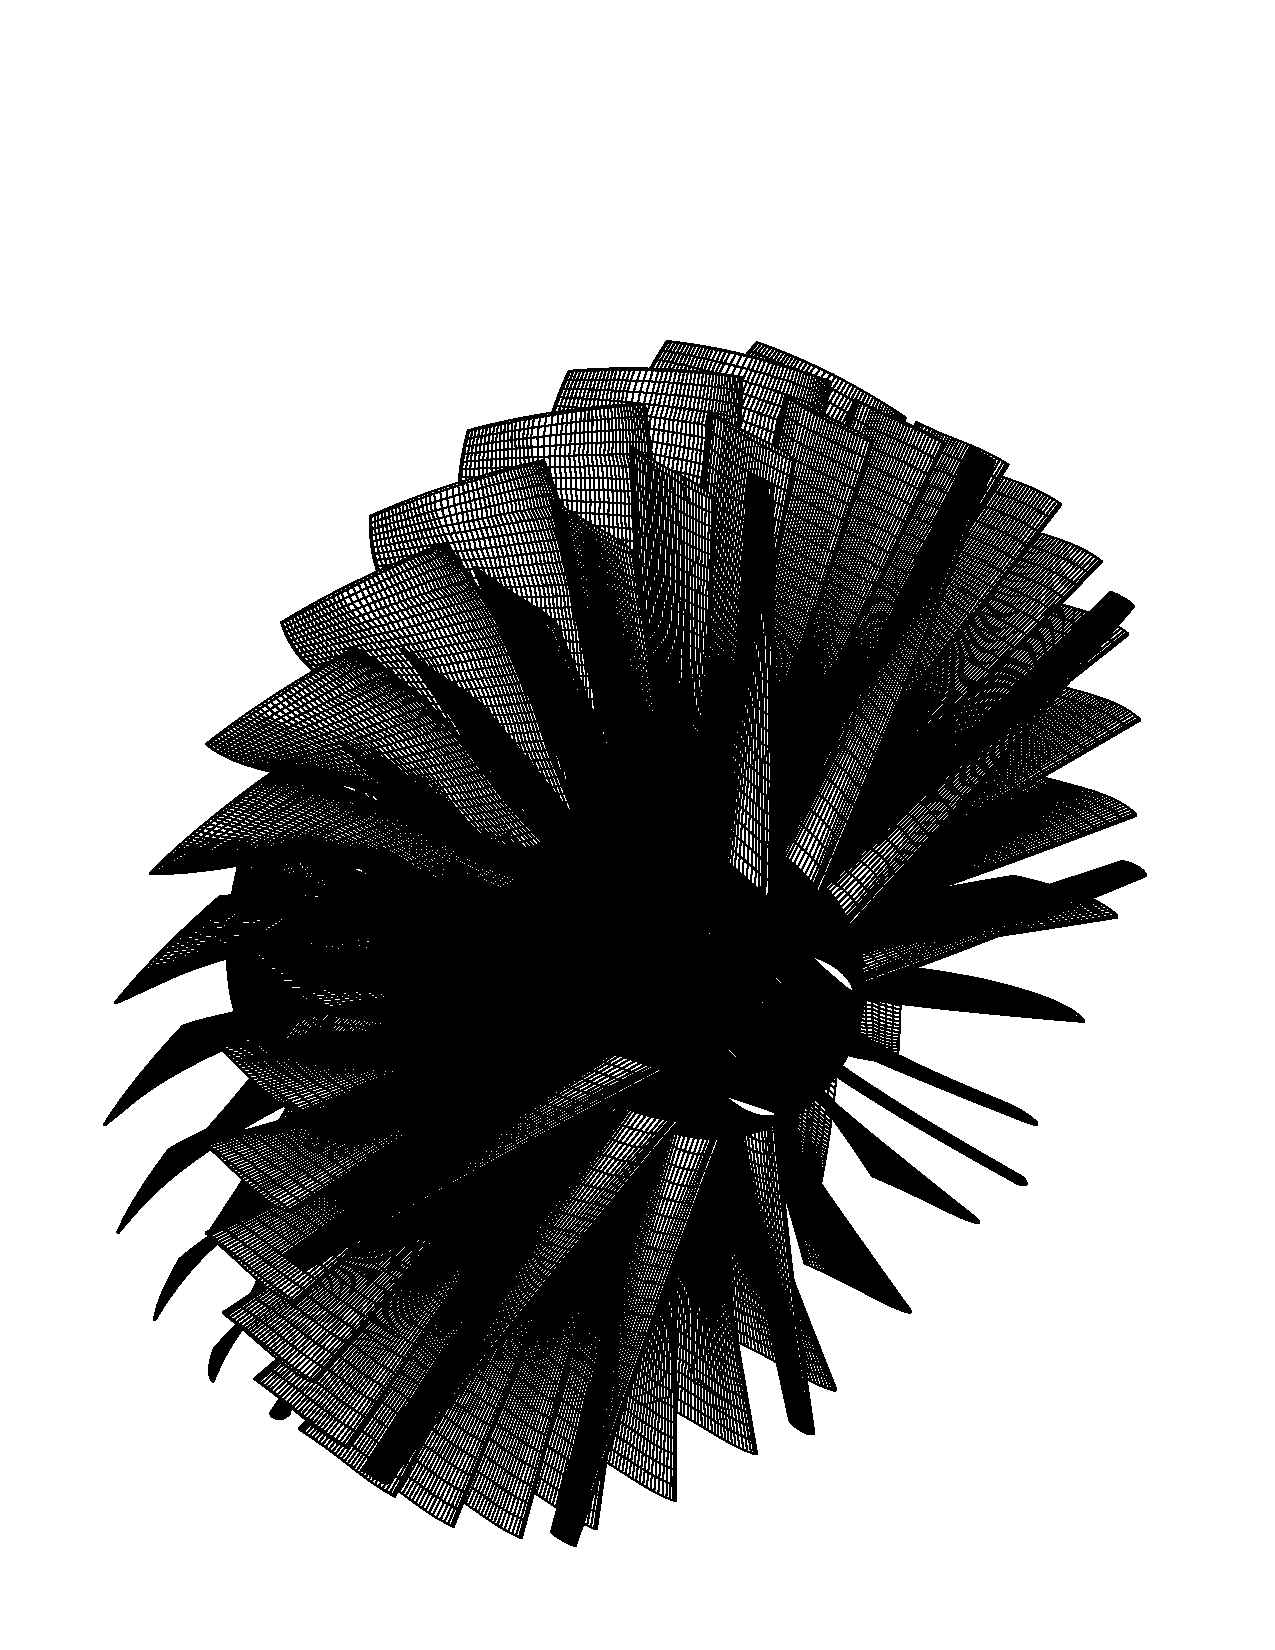
\includegraphics[width=120mm,clip=t]{CHAP_INTRO/FIGURE/threerows.pdf}}
  \caption{Three blade rows computational mesh for a 11 struts, 33 VIGVs and
           36 rotor blades (from Sayma et al. 1999)}
  \label{threerows.fig}
\end{figure}
%
